% CMSB 2014 poster - BioPreDyn project
\documentclass[portrait,a1,usenames,dvipsnames]{sciposter}
\usepackage{color}
\usepackage[pdftex]{graphicx}
\usepackage{listings}
\usepackage{multicol}

\begin{document}

\conference{{\bf CMSB 2014}, 12th Conference on Computational Methods in
Systems Biology, 17-19 November 2014, University of Manchester, UK}
\leftlogo{fp7_logo.pdf}
\rightlogo{biopredyn_logo.pdf}
\title{BioPreDyn software: an implementation of the systems biology model
building cycle}
\author{Bertrand Moreau \& Eric Boix}
\institute{The CoSMo Company, Lyon, France}
\email{bertrand.moreau@thecosmocompany.com}
\maketitle

\begin{abstract}
Many methods and tools have been developed that deal with specific steps of
the systems biology model building cycle for data-driven computational models
\cite{Kitano2002}: data analysis, model building, parameter estimation,
identifiability analysis, uncertainty quantification, model discrimination, and
optimal experimental design. There is still a need for a software platform
supporting the entire cycle though; the BioPreDyn project aims at developing
such a platform. In this paper, we present an integrative software framework
for reading and executing workflows written using the Simulation Experiment
Description Markup Language (SED-ML). Current version handles workflows
combining simulation run, flux balance analysis and parameter estimation; its
application programming interface (API) also provides tools for assessing the
quality of a numerical model.
\end{abstract}

\begin{multicols}{2}

\section{Introduction}
In the scope of the BioPreDyn project, a simulation workflow - or
numerical experiment - is defined as a sequence of instructions to be executed
on a numerical model; instructions encoded in the workflow include model
initialization, simulation runs and result processing.

\begin{figure}
\begin{minipage}[c]{0.5\textwidth}
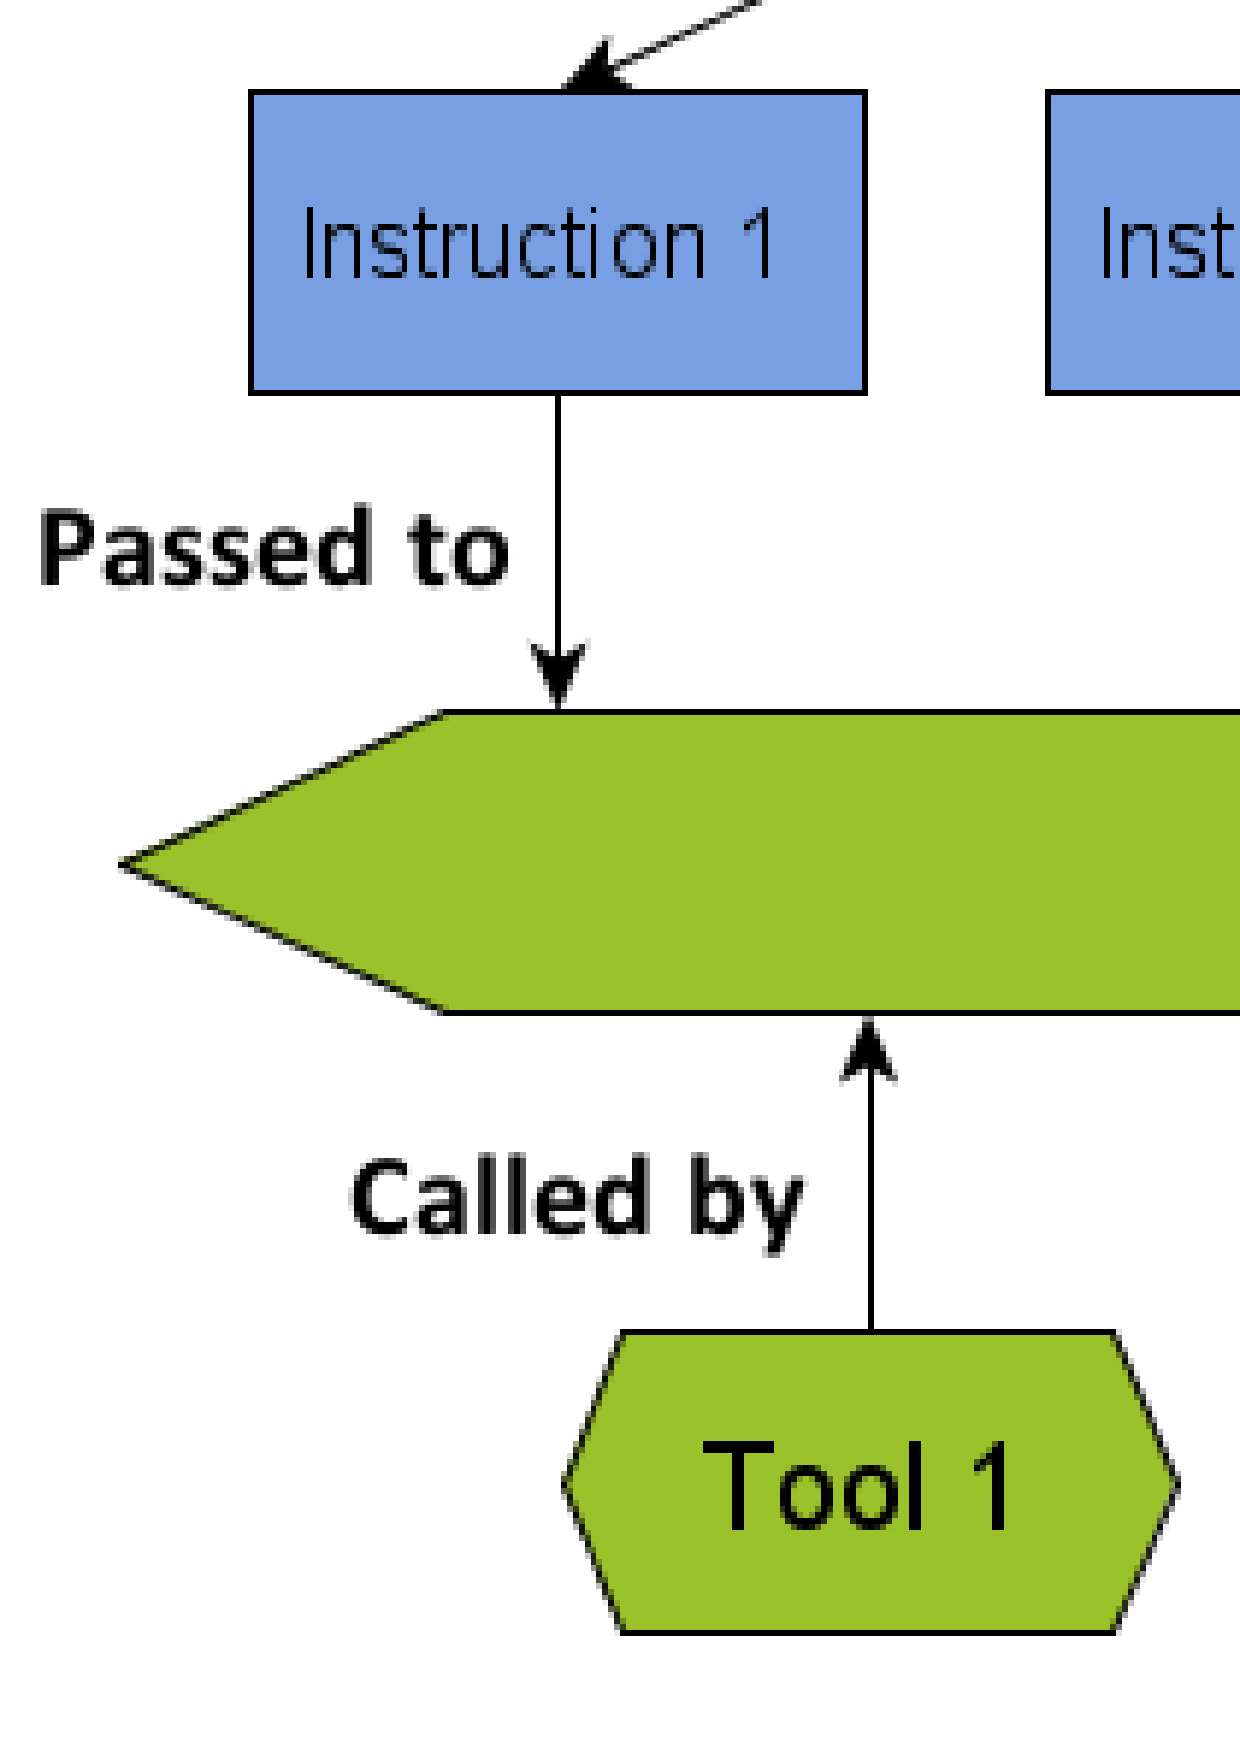
\includegraphics[width=\textwidth]{proposal_complete.pdf}
\end{minipage}\hfill
\begin{minipage}[c]{0.45\textwidth}
\caption{Representation of a simulation workflow in BioPreDyn: a parser reads
the workflow from its physical representation and passes it to the engine as a
series of instructions; each instruction describes an operation and refers to
a model. The engine dispatches the instructions to the appropriate tools and
schedules their execution following the order specified in the input workflow
file.}
\end{minipage}
\end{figure}

In this context, "executing a workflow" simply means executing each instruction
sequentially. The following standard languages were chosen to describe the
various elements composing a generic model building workflow:
\begin{enumerate}
\item As a workflow description language: Simulation Experiment Description
Markup Language (SED-ML);
\item As a modeling language: Systems Biology Markup Language (SBML);
\item As a numerical result description language: Numerical Markup Language
(NuML), derived from the Systems Biology Results Markup Language (SBRML).
\end{enumerate}

\section{Implementation}
With those requirements in mind, an open-source software framework hosted on the
GitHub platform was developed. This implementation consists of:
\begin{enumerate}
\item A Python API allowing users to create and edit simulation workflows;
\item Parsers for reading workflows from SED-ML files, describing the tasks,
and passing them to the simulation engine;
\item A Python-based engine capable of dispatching the tasks read by the parsers
to the corresponding simulation tools;
\item A collection of simulation libraries and tools, capable of performing one
or more of the systems biology model building cycle steps.
\end{enumerate}
The BioPreDyn software relies on several tools for writing or reading specific
file formats, running simulations, accessing data bases, etc: dedicated parsers
(libSEDML, libSBML, and libNuML respectively for SED-ML, SBML and NuML files),
simulation engines (libSBMLSim\cite{Takizawa2013}, CobraPY\cite{Ebrahim2013}
and COPASI\cite{Hoops2006}), web services (BioServices\cite{Cokelaer2013}).
Depending on the task to be done, the user can therefore choose between
different simulation engines.

\section{Usage}
The BioPreDyn software can be used as any Python library for scripting more
elaborated workflows:
\lstinputlisting[
  language=Python,
  basicstyle=\footnotesize\ttfamily,
  keywordstyle=\color{ForestGreen},
  commentstyle=\color{Gray},
  stringstyle=\color{Fuchsia}]{script_example.py}
\bibliography{references}{}
\bibliographystyle{splncs03}
\end{multicols}
\end{document}
